%%---------------------------------------------------------------------
%	Preamble
%	Semesterprojekt 4 - gruppe 1
%	IHA F17
%---------------------------------------------------------------------
\documentclass[12pt,fleqn,a4paper]{report}
\usepackage[utf8]{inputenc}
\usepackage[danish]{babel}
\usepackage[top=2.5cm, left=2cm, right=2cm, bottom=2.5cm]{geometry}
\usepackage{graphicx}
\usepackage[bottom]{footmisc}
\usepackage{framed}
\usepackage{caption}
\usepackage{float}
\usepackage{mdframed}
\usepackage{listings}
\usepackage{color}
\usepackage[T1]{fontenc}
\usepackage{amsmath,amsfonts,amsthm} % Math packages
\usepackage{array}
\usepackage{wrapfig}
\usepackage{multirow}
\usepackage{tabu}
\usepackage{longtable}
\usepackage{lastpage}
\usepackage{fancyhdr}
\usepackage[compact]{titlesec}
\usepackage[table,xcdraw]{xcolor}
\usepackage{arydshln}
\usepackage[style=ieee]{biblatex}

\definecolor{mygreen}{RGB}{28,172,0} % color values Red, Green, Blue
\definecolor{mylilas}{RGB}{170,55,241}
\renewcommand{\lstlistingname}{Kodeudsnit}
\tabulinesep=3mm

\setcounter{secnumdepth}{2}
\setcounter{tocdepth}{1}

\setlength{\parindent}{0mm} %intet indryk
\setlength{\parskip}{3mm} 	%linjeskift v. afsnit

% Ændring af enumerize og itemize 
\usepackage{enumitem} % @http://ctan.org/pkg/enumitem
\setlist[itemize]{topsep=0pt, itemsep=0.5pt}
\setlist[enumerate]{topsep=0pt, itemsep=0.5pt}

%afstand omkring sections
\titlespacing{\section}{0pt}{5mm}{0pt}
\titlespacing{\subsection}{0pt}{2mm}{0pt}
\titlespacing{\subsubsection}{0pt}{2mm}{0pt}

\usepackage{arydshln}
%aryd
\setlength\dashlinedash{3pt}
\setlength\dashlinegap{4pt}

\lstset{language=C++,
	breaklines=true,
	keywordstyle=\color{blue},
	stringstyle=\color{red},
	commentstyle=\color{mygreen},
	morecomment=[l][\color{magenta}]{\#}
}

%header & footer
\makeatletter
\pagestyle{fancy}
\fancypagestyle{plain}{}
\renewcommand{\chaptermark}[1]{\markboth{#1}{}}
\setlength{\headheight}{35pt}
\fancyfoot{} % clear all fields
\fancyfoot[R]{Side \thepage\ af \pageref{LastPage}}
\fancyhead{} % clear all fields
\fancyhead[L]{\includegraphics[clip, trim = 0 0 240pt 0, height=30pt]{Figur/IHA_AU_logo.png}}
\fancyhead[R]{\includegraphics[height = 30pt]{Figur/logo.png}}
\fancyhead[C]{\ifnum\value{chapter}>0 \leftmark \fi}
\renewcommand{\headrulewidth}{0pt}

\def\thickhrulefill{\leavevmode \leaders \hrule height 1.2ex \hfill \kern \z@}
\def\@makechapterhead#1{
  \vspace*{10\p@}%
  {\parindent \z@ \centering \reset@font
        \thickhrulefill\quad 
        \scshape\bfseries\textit{\@chapapp{}  \thechapter}  
        \quad \thickhrulefill
        \par\nobreak
        \vspace*{10\p@}%
        \interlinepenalty\@M
        \hrule
        \vspace*{10\p@}%
        \Huge \bfseries #1 \par\nobreak
        \par
        \vspace*{10\p@}%
        \hrule
        \vskip 40\p@
  }}



\graphicspath{ {Figur/} }


%Se Kodeudsnit \ref{lstlisting:generel_kode}

%\captionof{lstlisting}{Generelle egenskaber for koden til fremstilling af diverse figure i matlab} 
%\label{lstlisting:generel_kode}
%\vspace{5mm} %5mm vertical space
%
%\subsection{Kode til lyd i forhold til tiden}
%\begin{framed}
%\begin{center}
%\begin{lstlisting}
%figure('name','trafikstoejen i fuld laengde'); clf
%subplot(211);
%plot(t,s_sound_left)
%xlabel('Tid (sek)')
%ylabel('Signalstyrke')
%title('Trafikstoej set i forhold til tiden')
%grid on
%hold on
%\end{lstlisting}
%\end{center}
%\end{framed}



%\begin{document}
	
%---------------------------------------------------------------------
%	SYSTEMARKITEKTUR
%---------------------------------------------------------------------
\chapter{Systemarkitektur}

\section{Hardwarearkitektur}
Dette afsnit beskriver systemets hardwarearkitektur ved brug af sysML værktøjerne BDD og IBD. 

\subsection{BDD}
Figur \ref{fig:BDD_system} viser de overordnede blokke, systemet består af.
\begin{figure} [H]
	\centering
	\includegraphics[clip, trim = 0cm 0cm 0cm 0.5cm ,width = 0.7 \textwidth]{figur/BDD_eyeRobot.pdf}
	\caption{Overordnet blokdiagram for hele systemet}
	\label{fig:BDD_system}
\end{figure}
\newpage

\subsection{IBD}
Figur \ref{fig:IBD_robot} viser en intern blokbeskrivelse for robotten.
\begin{figure}[H]
	\centering
	\includegraphics[clip, trim = 0.5cm 0.5cm 0.5cm 1cm ,width = \textwidth]{figur/IBD_robot.pdf}
	\caption{internt blokdiagram for robotten}
	\label{fig:IBD_robot}
\end{figure}

I bilag \ref{appendix:signalbeskrivelse} er systemets signaler beskrevet i en signaltabel. I tabellen er signalernes funktion og hvilke porte de løber mellem beskrevet. I tabellen er der også beskrevet signalernes spænding og strøm niveauer, sammen med eventuel yderligere information.  



\newpage
\section{Softwarearkitektur}
Dette afsnit beskriver systemets softwarearkitektur ved brug af en domæneanalyse, samt UML værktøjerne sekvensdiagram, tilstandsdiagram og klassediagram. 

\subsection{Domæneanalyse}
Domæneanalysen på figur \ref{fig:Domainmodel} viser koncepterne i systemet og hvordan de interagerer. Domænemodellen bruges til at identificere de software klasser systemet består af. 

\begin{figure}[H]
	\centering
	\includegraphics[width = \textwidth]{figur/Domainmodel.pdf}
	\caption{Domænemodel for systemet EyeRobot}
	\label{fig:Domainmodel}
\end{figure}

\newpage

\subsection{Aktør- og blokbeskrivelse}

Aktør:
\begin{itemize}
	\item{Bruger - Personen, der styrer robotten med sine øjne.}
\end{itemize}

Blokke:
\begin{itemize}
	\item{PC             - Indeholder EyeRobot applikationen}
	\item{PC-Kamera      - Optager brugerens ansigt}
	\item{Aktivt valg    - Registerer om brugeren har foretaget et aktivt valg}
	\item{GUI            - Styrer, hvad der vises på PC'ens skærm}
	\item{Wifi           - Kommunikationsvej mellem PC og robot}
	\item{Kontrolenhed   - Kommunikerer med motorkontrolenheden over I2C, kommunikerer med PC'en over Wifi og streamer videofeed fra robotkamera}
	\item{Motorkontrolenhed  - Styringsenheden der sørger for at robotten kan køre}
	\item{Robotkamera   - Optager videofeed i køreretning}
	\item{Motorer        - Giver robotten bevægelighed}
	
\end{itemize}
\newpage

\subsection{Allokering}
Systemet består af forskellige logiske enheder. 
Disse enheder befinder sig i forskellige fysiske dele af systemet. 
På figur \ref{fig:allokeringsdiagram} kan det ses, hvilke CPU’er de logiske enheder er allokeret på.  

\begin{figure}[H]
	\centering
	\includegraphics[width = \textwidth]{figur/allokeringsdiagram.pdf}
	\caption{Allokeringsdiagram for systemet EyeRobot}
	\label{fig:allokeringsdiagram}
\end{figure}
\newpage


\subsection{Applikationsmodeller}
Dette afsnit beskriver softwarearkitekturen for CPU'erne i systemet, ved brug af applikationsmodeller. 

\subsubsection{PC Applikationsmodel}
PC'en har til ansvar at udføre øjendetektering. 
Ud fra dette skal PC'en opdatere GUI'et og sende beskeder til robotten. 
Derudover skal den også kunne modtage data fra robotten. 
Dataen indebærer et videofeed, der skal vises på GUI'et, samt information om robottens tilstand, der bruges til at opdatere GUI'et. \\ 
For yderligere information om PC'ens funktionalitet henvises til bilag \ref{appendix:Applikationsmodeller}. 
Heri findes sekvensdiagrammer samt tilstandsdiagrammer for PC'en. 

Ud fra diagrammerne i bilaget er følgende klassediagram lavet.

\begin{figure}[H]
	\centering
	\includegraphics[width = \textwidth]{figur/classPCVisioFil.pdf}
	\caption{Klassediagram for PC'en}
	\label{fig:klassediagramPC}
\end{figure}

\newpage
\subsubsection{Kontrolenhed Applikationsmodel}
Kontrolenheden har til ansvar at videresende modtagne beskeder og streame et videofeed fra robotkameraet til PC'en over WiFi forbindelsen. \\ 
For yderligere information om Kontrolenhedens funktionalitet henvises til bilag \ref{appendix:Applikationsmodeller}. 
Heri findes sekvensdiagrammer for Kontrolenheden.

Ud fra diagrammerne i bilaget er følgende klassediagram lavet.

\begin{figure}[H]
	\centering
	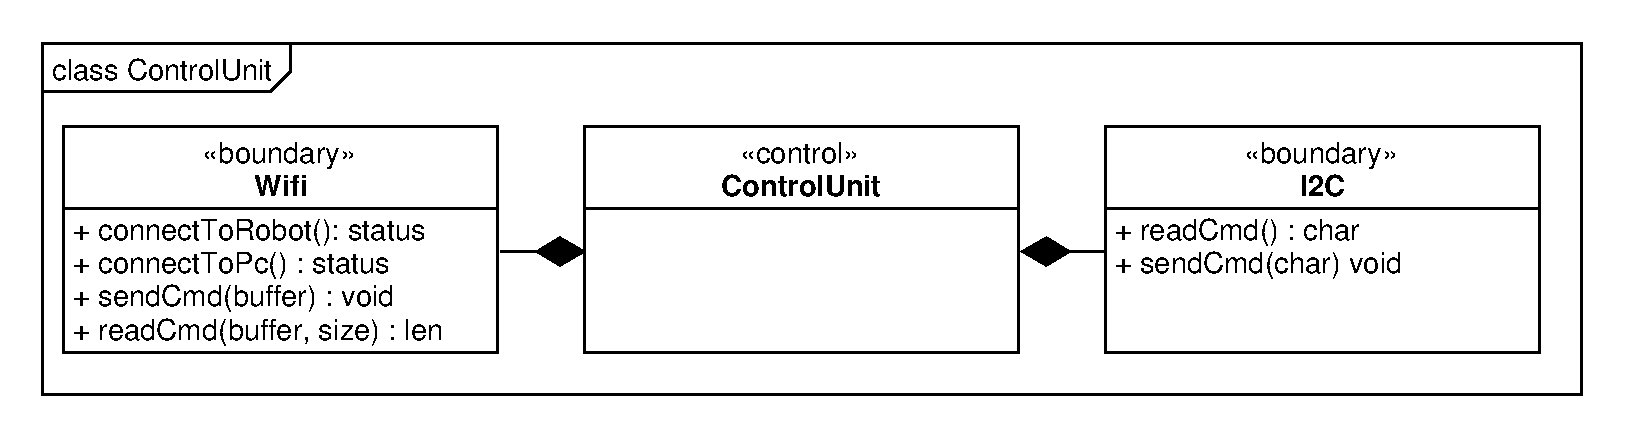
\includegraphics[width = \textwidth]{figur/classCUUdfyldt.pdf}
	\caption{Klassediagram for Kontrolenheden}
	\label{fig:klassediagramCU}
\end{figure}


\subsubsection{Motorkontrolenhed Applikationsmodel}
Motorkontrolenheden har til ansvar at kontrollere robottens motorer ud fra input fra Kontrolenheden. 
Motorkontrolenheden har også til ansvar at informere Kontrolenheden om, hvorvidt robotten er i bevægelse eller er stoppet. 
Derudover regulerer den robottens motorer. \\ 
For yderligere information om Motorkontrolenhedens funktionalitet henvises til bilag \ref{appendix:Applikationsmodeller}, der indeholder et tilstandsdiagram.

Ud fra diagrammerne i bilaget er følgende klassediagram lavet.

\begin{figure}[H]
	\centering
	\includegraphics[width = \textwidth]{figur/classMCVisioFil.pdf}
	\caption{Klassediagram for Motorkontrolenheden}
	\label{fig:klassediagramMC}
\end{figure}

\pagebreak
\subsection{Protokol beskrivelse}
I dette afsnit findes en beskrivelse af systemets kommunikationsformer og beskederne der sendes mellem enhederne. 
De valgte kommunikationsformer ses på figur \ref{fig:kommunikationsOversigt}.

\begin{figure}[H]
	\centering
	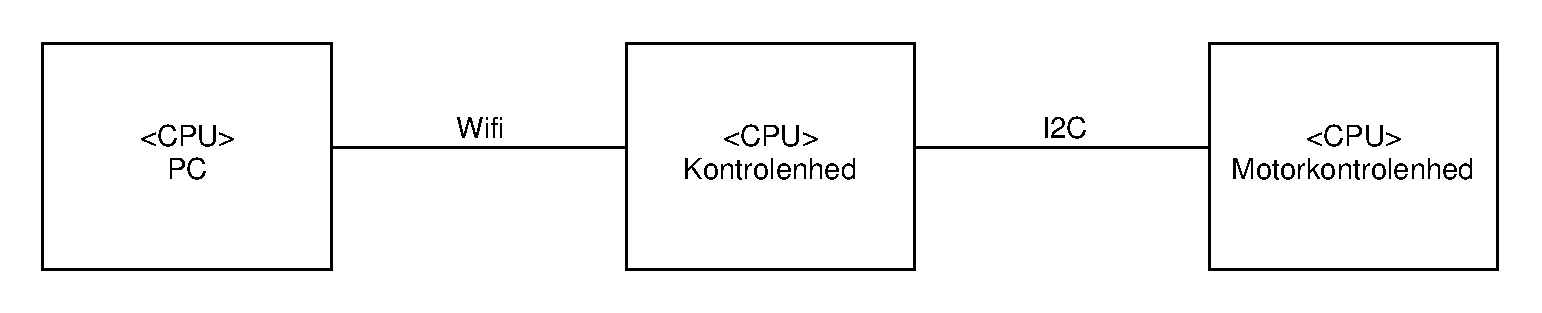
\includegraphics[width = \textwidth]{figur/ProtokolBeskrivelse.pdf}
	\caption{Oversigt over kommunikation mellem enhederne}
	\label{fig:kommunikationsOversigt}
\end{figure}


\subsubsection{Wifi}
Til kommunikation og videostreaming mellem PC og Kontrolenhed er det valgt at anvende wifi. 
Wifi vælges da det har en lang rækkevidde og er indbygget i både PC og Pi. 
Derudover giver det mulighed for at anvende transport protokollerne TCP og UDP.

\begin{figure}[H]
	\centering
	\includegraphics[width = \textwidth]{figur/Design_concept_simple.png}
	\caption{Oversigt over kommunikation mellem enhederne}
	\label{fig:Design_concept_simple}
\end{figure}

Pi'en opsættes som et hotspot, som PC'en skal forbindes til for at kommunikere med den, mere om dette kan læses i designafsnittet om Kontrolenheden.

Til videostreamingen anvendes en afart af UDP. 
UDP er en upålidelig protokol, men den er valgt til overførsel af videofeedet, da pakker derved bliver kasseret, hvis der sker en fejl i transmissionen. 
Hvis der i stedet var anvendt TCP ville der komme delay i videostreamet i tilfælde af tabte pakker. 
Derudover er UDP den hurtigste af transportprotokollerne TCP og UDP, hvilket giver den mindste forsinkelse i streamen. \\
Alle datapakker, der sendes over UDP, valideres med en checksum. 
Dataene antages derfor korrekte, hvis de går gennem valideringen. 

Til overførsel af kommandoer anvendes TCP. 
TCP anvendes, da det er en pålidelig protokol, som sikrer at kommandoerne overføres. \\
TCP - samt UDP - vælges desuden, fordi gruppen har erfaring med at arbejde med disse to protokoller.

\newpage
\subsubsection{I2C}
Til kommunikationen mellem Kontrolenheden og Motorkontrolenheden anvendes I2C protokollen. 
I2C er valgt, fordi det er en hurtig kommunikationsbus, der kun bruger to ledninger og er let udvidbar. 
Det er nødvendigt for kommunikationslinjen at være udvidbar, da det også er denne linje, der bruges til kommunikation med udvidelsesmoduler. 
Gruppen har desuden erfaring med at arbejde med I2C.\\
I2C er ikke en pålidelig protokol, så der kan forekomme fejl i beskederne under overførsel. 
I2C har ingen yderligere validering, da der ved I2C brug i for eksempel Linux kernen ikke er nogen validering.
Der bliver i stedet taget højde for fejl i beskedopbygningen.\\ 
I2C er opsat med en datarate på 100kbps.


\subsubsection{Beskedopbygning}
Dette afsnit beskriver de beskeder, der sendes gennem systemets kommunikationslinjer. 
Alle beskederne i systemet er opbygget med det formål at mindske risikoen for, at en besked bliver forvekslet med en anden besked.  \\
For Wifi beskederne er dette gjort ved at skrive hele ord, hvilket øger sandsynligheden for at fejl i beskederne opdages af TCP-checksummen.
Tabel \ref{Wifi_Beskedopbygning} viser beskedopbygningen for Wifi beskederne.\\
For I2C beskederne er risikoen for fejl mindsket ved, at mindst to bits skal fejle samtidigt, for at beskederne kan forveksles.
Tabel \ref{I2C_Beskedopbygning} viser beskedopbygningen for I2C beskederne.


\begin{table}[H]
	\centering
		\begin{tabu} to 1 \textwidth { X[l,3]  X[l,1] X[l,3]}
			\hline
			\multicolumn{3}{c}{Beskeder fra PC til Kontrolenhed}\\
			\hline
			\textbf{Define}  	&  \textbf{Besked} 	&  \textbf{Kommentar} \\
			\hdashline
			RobotMsg\_forward  	& forward 	&  Kør fremad \\
			\hdashline
			RobotMsg\_left  	& left 		&  Drej venstre om \\
			\hdashline
			RobotMsg\_right 	& right 	&  Drej højre om \\
			\hdashline
			RobotMsg\_brake  	& brake 	&  Brems \\
			\hdashline
			RobotMsg\_neutral  	& neutral 	&  Frigear \\
			\hdashline
			RobotMsg\_slumber  	& slumber 	&  Gå i dvale \\
			\hdashline
			RobotMsg\_start  	& start 	&  Start \\
			\hline
			\multicolumn{3}{c}{Beskeder fra Kontrolenhed til PC}\\
			\hline
			RobotMsg\_stopped  		& stopped 			&  Robot stoppet \\
			\hdashline
			RobotMsg\_moving  		& moving 			&  Robot i bevægelse \\
			\hdashline
			RobotMsg\_slumber\_ack 	& slumber\_ack 		&  Robot gået i dvale \\
			\hline
		\end{tabu}
	\caption{Beskedopbygning for beskederne der sendes over Wifi}
	\label{Wifi_Beskedopbygning}
\end{table}


\begin{table}[H]
	\centering
		\begin{tabu} to 1 \textwidth { X[l,3]  X[l,1] X[l,3]}
			\hline
			\multicolumn{3}{c}{Beskeder fra Kontrolenhed til Motorkontrolenhed}\\
			\hline
			\textbf{Besked}  	& \textbf{Binær} 	&  \textbf{Kommentar} \\
			\hdashline
			Control\_left\_message  	& 0b10000001 	&  Får robotten til at dreje venstre om \\
			\hdashline
			Control\_right\_message  	& 0b00000011 	&  Får robotten til at dreje højre om \\
			\hdashline
			Control\_forward\_message  	& 0b00001111 	&  Får robotten til at køre ligeud \\
			\hdashline
			Control\_brake\_message  	& 0b00111111 	&  Får robotten til at bremse \\
			\hdashline
			Control\_neutral\_message  	& 0b11110111 	&  Sætter robotten til at køre i frigear \\
			\hdashline
			System\_sleep\_message  	& 0b11000000 	&  Sætter robotten i dvaletilstand \\
			\hdashline
			System\_start\_message  	& 0b11110000 	&  Får robotten til at vågne fra dvaletilstand \\
			\hline
			\multicolumn{3}{c}{Beskeder fra Motorkontrolenhed til Kontrolenhed}\\
			\hline
			robot\_stopped\_message   	& 0b11111100 	&  Indikerer at robotten er stoppet \\
			\hdashline
			robot\_moving\_message  	& 0b11111100 	&  Indikerer at robotten er i bevægelse \\
			\hline	
		\end{tabu}
	\caption{Beskedopbygning for beskederne der sendes over I2C}
	\label{I2C_Beskedopbygning}
\end{table}




%\end{document}